
\begin{figure*}
    \centering
            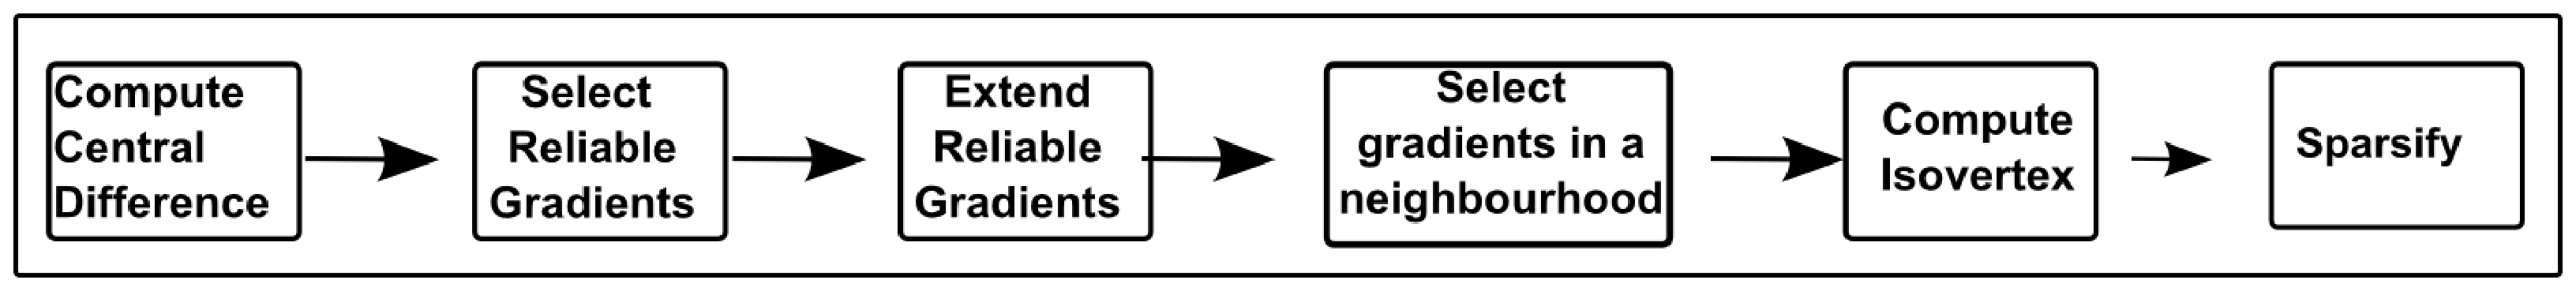
\includegraphics[width=\linewidth]{images/flowchartCrop3.eps}
\caption{Constructing points on sharp features.}
\label{fig:flowchart}
\end{figure*}


\firstsection{Introduction}

X-ray computed tomography (CT) scanners produce regular grids
of scalar values representing material densities of scanned objects.
These scalar values can be modeled as samples of some scalar field
$f:\Rthree \rightarrow \R$.
Object boundaries can be visualized by direct volume rendering
or by visualizing isosurfaces (mesh representations of $f^{-1}(\sigma)$)
representing the object boundaries.
Both approaches have difficulties in representing sharp edges and corners
in the object boundaries.
Sharp edges and corners are best represented
as discontinuities in the gradient field of $f$.
However, standard direct volume rendering 
and isosurface construction algorithms implicitly assume
some continuity in the gradient field of $f$.

In this paper,
we will describe a fast, local algorithm for reliably reconstructing
the gradient field of $f$ 
and constructing points on sharp edges and corners of an isosurface.
The points can be rendered in conjunction with isosurface visualizations
to highlight sharp features or
they can be joined to form a skeleton representation of the sharp feature.
They can also be used as input to isosurface or surface meshing algorithms
which are designed to handle surfaces with sharp features.

Previous algorithms to construct isosurfaces with sharp features
relied upon exact surface normals being provided 
to the algorithm~\cite{
ab-fpmmo-03,gk-eretm-04,hwco-cmsaf-05,jlsw-dchd-02,
kbsh-fssev-01,ms-ispmg-10,Varadhan:2003:fss,sw-dmcpc-04,zhk-dctps-04}.
The algorithm in~\cite{bw-cisec-13}
constructs isosurfaces with sharp features
from gradient grid data
where gradients are provided at each grid vertex.
We know of no work on constructing isosurfaces with sharp features
directly from scalar data.

If the level set $f^{-1}(\sigma)$ of a scalar field
$f:\Rthree \rightarrow \R$ has sharp features,
then there are discontinuities in the gradients of $f$
at the sharp features.
Constructing the gradients near those discontinuities
is difficult.
Formulas for approximating gradients
such as the central difference formula~\cite{ck-nmc-07}
or higher order approximations~\cite{aml-ger-10,ham-thqge-11,mmmy-cnes-97}
assume the gradient is continuous at the given location.
Anisotropic diffusion~\cite{
bx-adsfs-03,cdr-agdsp-00,twbo-gssad-02,twbo-gspnm-03,tw-adsnf-03} 
removes noise in low curvature regions of the scalar field 
without affecting high curvature regions,
but it does not produce correct gradients near gradient discontinuities.

Instead of attempting to produce correct gradients at all grid vertices,
our algorithm identifies correct gradients 
and uses only those gradients to predict locations
of isosurface vertices.
We give an algorithm for identifying correct gradients
based on their agreement with neighboring gradients.
The algorithm produces enough correct gradients in the neighborhood
of sharp features to generate points on those sharp features.

The basic steps of our algorithm are given in Figure~\ref{fig:flowchart}.
The first two steps produce a set of reliable gradients.
The algorithm then selects a set of reliable gradients around each cube,
computes a set of isosurface tangent planes from those gradients,
and finds a point at the ``intersection'' of those tangent planes.
It simultaneously identifies whether that point lies 
on a sharp edge or corner of the isosurface
or on a smooth region of the isosurface.
The algorithm sparsifies the set of isosurface vertices on sharp features
and returns the sparsified set.
The sparsified set can be used for generating an isosurface mesh
using feature preserving algorithms such as MergeSharp~\cite{bw-cisec-13}
or Weighted Cocone~\cite{dgqsww-fprss-12}.
Alternatively, it can be used to construct a representative sharp
feature curve or can be rendered directly to highlight sharp features
on the isosurface.

The focus of this paper is on constructing a set of reliable gradients
from scalar data in the presence of gradient discontinuities.
As part of our work, we developed a theory (Section~\ref{sec:gradients} 
giving bounds on gradient approximation errors
based on comparing gradients to nearby gradients.

There is a substantial amount of work on computing surfaces 
with sharp features from point cloud data.
Some of the proposed algorithms (e.g. \cite{dgqsww-fprss-12,sym-fpmg-10})
compute points on sharp features
and then create representative curves from those points.
Scalar data might be turned into point cloud data 
by computing a set of points which approximate the
intersection of the isosurface and the grid edges.
Any of the point cloud algorithms which reconstruct sharp features 
or surfaces with sharp features can then be applied to this point cloud data.

We strongly believe that there is a big advantage in constructing sharp features
directly from scalar data without (the extra step of) converting it to point cloud data.
First, converting scalar data to point cloud data ignores the grid structure
of the scalar data.
This grid structure can be employed both for constructing sharp features
and for meshing those features. Generally, grid based methods are faster than their point-cloud counterparts.
Second, point cloud data is extremely noisy so the point cloud 
reconstruction algorithms average over \textit{large} neighborhoods.
It is extremely difficult to predict the results of the algorithms
or to guarantee that the algorithms are not ignoring features in the data.
In contrast, our algorithm runs over a small, local neighborhood,
so that all features of the data (for better or for worse) are represented in the output.
Finally, because our algorithm is local,
it is very fast and easily parallelizable.

Our research contributions in this paper are:
\begin{enumerate}
\itemsep0em 
\item An algorithm for constructing reliable gradients
from scalar data in the presence of gradient discontinuities.
\item Proofs of bounds on the angle between the approximate gradients
and the true gradients.
\end{enumerate}
We use our algorithm to:
\begin{enumerate}
\itemsep0em
\item Construct samples points on sharp edges and corners of an isosurface.
\item Construct isosurface meshes with good representations of sharp edges and corners.
\end{enumerate}

We note that the algorithm for constructing the reliable gradients and the sample points
is completely local, and thus fast and easily parallelizable.






